\documentclass[12pt]{article}
\usepackage[top=1.125in, bottom=1.125in, left=0.85in, right=0.85in]{geometry}
\usepackage[utf8]{inputenc} % Required for inputting international characters
\usepackage[T1]{fontenc} % Output font encoding for international characters
\usepackage{setspace} % Simplify line spacing with 'spacing' command (see below)
\usepackage[table]{xcolor} % Define custom colors
\usepackage{longtable} % Create tables that span multiple pages
\usepackage{multirow} % Create cells spanning multiple rows or columns
\usepackage{mdframed} % Framed environments that can split at page boundaries
\usepackage{minted} % Code highlighting
\usepackage{changepage}
\usepackage{graphicx}
\usepackage{multicol}
\setlength{\columnsep}{0.25in}
\graphicspath{ {./img/} }
\usepackage{makecell} % Allows for more formatting options within table cells
\usepackage{caption}% Allows for captions to be made for figures/images
\usepackage[backend=biber]{biblatex} % References library
\bibliography{references}

% General formatting
\newcommand{\paragraphheaderspace}{8pt}
\newcommand{\eqnspace}{-24pt}
\definecolor{bgcolor}{RGB}{230,236,247}

% Table formatting
\newcommand{\cellpaddingvertical}{1.05}
\newcommand{\tablehead}[1]{\bfseries \cellcolor{bgcolor} #1}
\renewcommand\cellalign{lc}

% Define 'htmlcode', 'jsoncode', and 'javascriptcode' minted code style shortcuts
\newminted{html}{}
\BeforeBeginEnvironment{htmlcode}{\begin{mdframed}[backgroundcolor=bgcolor,topline=true,bottomline=true,rightline=false,leftline=false]}
\AfterEndEnvironment{htmlcode}{\end{mdframed}}
\newminted{json}{}
\BeforeBeginEnvironment{jsoncode}{\begin{mdframed}[backgroundcolor=bgcolor,topline=false,bottomline=false,rightline=false,leftline=false]}
\AfterEndEnvironment{jsoncode}{\end{mdframed}}
\newminted{javascript}{}
\BeforeBeginEnvironment{javascriptcode}{\begin{mdframed}[backgroundcolor=bgcolor,topline=false,bottomline=false,rightline=false,leftline=false]}
\AfterEndEnvironment{javascriptcode}{\end{mdframed}}
% Use this for small code snippets in need of minor formatting, e.g. var names
\newcommand{\codesnip}[1]{\mintinline{html}{#1}}

\begin{document}
  \begin{multicols*}{2}
    \begin{center}
  {\LARGE Mangrove}\\
  \vspace{5mm} %5mm vertical space % Title of your document
  {\Large Soundscape Ecology Analysis Toolkit}\\
  \vspace{5mm} %5mm vertical space % Title of your document
  {\fontsize{12}{14} David Palumbo, Brita Ramsay, Joshua Pollmann, Ot Gabaldon Torrents, Keith Guske}\\
  \vspace{5mm} %5mm vertical space
  {\fontsize{12}{14} Department of Computer Science, University of Central Florida, Orlando, Florida, 32816-2450}\\
\end{center}

    \begin{flushleft}
  \setlength{\parindent}{0.125in}
  {\setstretch{0.7}
    {\indent\fontsize{9}{11}\bfseries
      \par\textit{Abstract}  -- Researching soundscape ecology requires a large amount of data in the form of sound files. Sound files demand both digital space and processing power to analyze and draw conclusions from them. Mangrove provides a free and open-source software suite that simplifies the job of organizing and analyzing audio recordings of natural soundscapes using existing algorithms in the field of soundscape ecology. The results of these algorithms are used to create interactive data visualizations. Using these visualizations, researchers are able to come to conclusions regarding their research points, all while providing visual representations of these conclusions.
    }
    \par{\fontsize{9}{11}\bfseries
      \textit{Index Terms}  -- Ecology, Soundscape
    }
  }
  \vspace{10mm} %5mm vertical space
\end{flushleft}

    The field of soundscape ecology has made astounding progress in the last decade.
Recordings and new techniques have allowed for the gathering of massive amounts of sound data. While this remains good news for the field, it raises new problems. Who or what will listen to these recordings, and how can they be analyzed in an efficient way? Many techniques have cropped up, most prominent of which is having hired experts listen to recordings, but the technique we are focused on in this project are the use of indices. These indices are algorithms that can be run on sound files, which then produce numerical values that can uncover generalizations about the sound (more information be found in the Soundscape Ecology Indices section).\par
While the soundscape ecology indices have great potential, they have not yet been rigorously tested and are currently in the process of being tried out in field studies. The main downfall of the indices is that they are used to compress vast amounts of data about the health of an environment into relatively few data points. This leads to a loss of information. Along with this lossy compression, sound files must also be cleaned before the indices can be properly used. The cleaning often involves chopping off certain frequency ranges or manually removing geophonic and anthrophonic sounds in the recording. This cleaning, combined with the already lossy nature of the indices, provides very rough numerical descriptions of the sound files, which have yet to be proven completely accurate in general circumstances.\par
Due to the nature of the indices, they are often used alongside another method to verify their accuracy. As mentioned previously, experts are often used, and this method is often costly and time-consuming.\par
In researching machine listening, our goal was to determine the best techniques and models that could be used to recognize species\textquotesingle\ sounds. While the methods listed in the following sections are quite robust, in the sense that they have high accuracy ratings when used, they cannot be used for general cases. Depending on the machine learning methodology, it may or may not become necessary to build a unique model for each species of bird, and this makes it less than ideal as a substitute for the indices, but an ideal technique for verifying the indices\textquotesingle\ results in a specific environment. We hope that future groups may take advantage of our research and put it to use in furthering the Mangrove application.\par
\begin{center}
	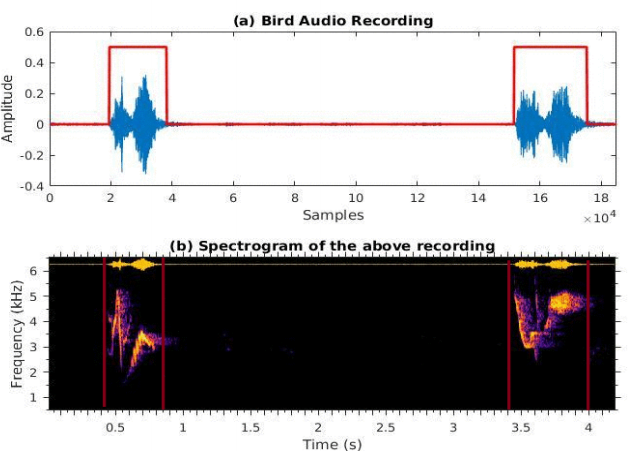
\includegraphics[width=.8\textwidth]{bird_spec}
\end{center}

    \subsection{Soundecology R Package Research}
The \codesnip{soundecology} R package was developed by Luis Villanueva. This package contains algorithms for calculating the major indices, along with some extra abilities. Obviously, each algorithm outputs the index value, however each also outputs specific values, value lists, and matrices that are also used heavily in this service for creating the visualizations.

\subsubsection{ACI Algorithm}
The ACI algorithm outputs more useful information than most of the other algorithms. In addition to the base ACI value, it outpus an ACI value by minute, which is a bit better representation of the ACI, especially for longer files. It also outputs a list of ACI values for each bin, which all sum up to the total ACI value. This list is useful for creating the line graphs included in this service. More information on the ACI index can be found in the Overview of Indices section.

\subsubsection{NDSI Algorithm}
The core NDSI algorithm that comes with the soundecology package outputs everything needed for this service, so no changes are needed. Those outputs include the NDSI values for both channels, as well as the biophony and anthrophony for both channels. These values are used for the visualizations, expanded upon in the Data Visualizations Research section.

\subsubsection{ADI and AEI Algorithm}
As ADI and AEI are closely related, their outputs are mostly the same, just tailored to the respective index. Along with the actual ADI or AEI value, the algorithms also output the ADI or AEI value for each band range, which is not included natively for AEI in the R package, and is included in the Proposed Changes section. These values include the ADI or AEI value at each frequency range, which can be specified by the user when creating jobs. Using these outputs, the ADI and AEI charts are able to be made.

\subsubsection{Bioacoustic Index Algorithm}
For the Bioacoustic index, the outputs for this service also include the left and right values, as well as the left and right normalized values for each frequency range. This is different than the base \codesnip{soundecology} package, and these changes are explained in the Proposed Changes section. For more information on how the Bioacoustic index is calculated, see the Overview of Indices section.

\subsubsection{Soundecology Package Dependencies}
The core soundecology package does not handle wav file conversion to Wav object that is needed for use in the algorithms. This is handled by a package named tuneR, which takes in audio files and converts them to R objects compatible with the R algorithms in soundecology. This is the only package that is of any note, as it will require its own set of instructions during our processing of the user\textquotesingle s files. The script for converting a user file into a Wav object is the following

\begin{javascriptcode}
  tdir <- getwd()
  tfile <- file.path(tdir, "SoundFileName.wav")
  newWobj <- readWave(tfile)
  result <- ndsi(newWobj)
\end{javascriptcode}

In order for this to work, the current working directory must be set to where the user\textquotesingle s files are located, and the SoundFileName must match the user\textquotesingle s as well. Luckily soundecology \textit{does} have a method, multiple_sounds, for going through all files in a subdirectory, and handles this natively. However multiple_sounds only goes through a directory, not for single file use.

\subsubsection{Proposed Changes}
For use in our service, this R package needs to be modified. Namely, the Bioacoustic index and AEI outputs need to be more detailed. For Bioacoustic, the bioacoustic values for both the left and right channels need to be output, along with the normalized left and right channel values. These values are in turn used in our visualizations to create the area graphs shown in the Data Visualizations Research section. As for AEI, it just needs to be changed to match that of the ADI. For whatever reason, the core package outputs only the AEI values for the left and right channel, and did not output the left and right band values and left and right band ranges. These are also used in the AEI and ADI visualizations.\par
Another proposed change that is talked about a bit in the Benchmarking section, is that of file size constraints. Currently, certain indices are not able to be computed on long files due to hardware limitations even on high end systems. These memory issues are the result of matrices being created in indices like ACI. From reviewing the code, these matrices are being used as intermediary values used in the calculation of lists of \textit{more} intermediary values. These matrices are in fact output to the user, however the usefulness of them is up for debate. Proposed changes to circumvent these issues include possibly removing these matrices, or adding a file splicing feature. Files that are over a certain length would need to be split into equal length parts, and the index would be calculated on each. From there, the overall index value could be calculated either in R or in the client.


    \begin{center}
II. Soundscape Indices
\end{center}
\begin{flushleft}
\setlength{\parindent}{0.125in}
The \codesnip{soundecology} R package was developed by Luis Villanueva. This package contains algorithms for calculating the major indices, along with some extra abilities. Obviously, each algorithm outputs the index value, however each also outputs specific values, value lists, and matrices that are also used heavily in this service for creating the visualizations.\par

\noindent\textit{A. Acoustic Complexity Index}\par
The ACI, in combination with other measuring techniques, can be a powerful tool for finding the Biophonic sounds within a recording. ACI relies on the fact that most Biophonic (non-human biological sounds) have a high level of complexity when it comes to their intensity. Meaning that most natural sounds have a high variance of loudness. This is in stark contrast with the mostly monotone nature of human made sounds. This key difference in sound types allows the ACI to filter out plane noises or car sounds amongst bird sounds and other Biophonic interests. While there is a promising amount of research for the ability of the ACI to discriminate between Anthrophony and Biophony, the algorithm still does very poorly in discerning between different types of Biophony and Geophony. This challenge can be highlighted by the fact that the algorithm produces high numbers for sounds such as buzzing insects and wind.\par

\noindent\textit{B. Normalized Difference Soundscape Index}\par
One goal within the field of soundscape ecology is the analysis of the key characteristics of the Anthropocene, that is, the impact that humans have on wildlife and Earth as a whole. And perhaps no other metric of analysis symbolizes this better than the NDSI. NDSI has the goal of measuring the ratio between anthropogenic sounds and biological sounds.\par
The basis of this metric originates from a 2004 thesis written by Brian Michael Napoletano entitled \textit{Measurement, Quantification and Interpretation of Acoustic Signals Within an Ecological Context.} In this paper, Napoletano proposed three classifications for the sources for domains of sound frequencies: geophony (full spectrum), anthrophony (0 to 2 kHz), and biophony (3 to 11 kHz).\cite{napoletano} By ignoring potential geophony (as it would occur over too wide of a spectrum to identify), NDSI measures the acoustic energy (in watts) produced within the anthrophony and biophony spectrums.\par
Of course, this metric has its limits. In addition to completely ignoring all signals of geophony, NDSI fails to take into account variations in acoustic energy patterns depending on the source of sound, the time of day, and the season.\par

\noindent\textit{C. Bioacoustic Index}\par
The bioacoustic index was originally developed by ecologists studying the effects of invasive species on the native bird population of Hawaii. The purpose of such an index was to create a metric that closely correlated to the actual population of birds within an environment. This way, the researchers could have a reasonable estimation of the amount of birds within a given area without having to count them all by hand all the time.\par
This metric works by first specifying a range of frequencies (in Hz) at which biophony (or just about any type of sound that researchers expect to target) is expected to occur. Then, within this range of frequencies, measure the power (in Db) produced from these recordings within bins of specified ranges of time (in s). This should result in a collection of segments of curves of power. Finally, through determining the average area underneath these curves, the bioacoustic index value is found.\par
Of course, however, this metric has some drawbacks. Namely, it requires knowledge of the environment that the field work is occurring in. In order for this metric to be used effectively, researchers need to know beforehand the frequency range they intend to target and the correlation factor between the actual population count and the bioacoustic index value.\par

\noindent\textit{D. Acoustic Evenness and Diversity Index}\par
The ADI (Acoustic Diversity Index) bases its numerical evaluation on the concept of evenness of a set. A statistical theory first appearing in the 1960\textquotesingle s it is used to measure the diversity of a set of data.\par
One of the great features of the ADI using the Shannon-Wiener index is that it is not greatly affected by sample size. Along with that the ADI can capture a lot of information in one expression. Which can be helpful to express data to a general audience. That being said you must put this index into context. Mainly one must state the range of values that the index can output. These minimum and maximum values put the output value into context for the data collected. Just like most indices it is important that diversity indices are used along other measures. This allows for a holistic measure of the state the environment is in.\cite{shannonWiener}\par
While the method of taking individual sounds of birds and using ratios of specific calls is much more accurate, it is very difficult to identify individual calls in an automated fashion. Thus, when using a script to calculate the evenness or diversity of a sound clip, bands of frequencies are often used.

\end{flushleft}

    \begin{center}
III. Mangrove Features
\end{center}
\begin{flushleft}
\setlength{\parindent}{0.125in}
The goal of our project is to provide a tool to researchers that will present data obtained by the R Soundecology package in a more accessible format. Mangrove uses the existing  algorithms to produce data from audio recordings and turn it into meaningful visualizations. Through Mangrove\textquotesingle s user interface, sound files, along with specifications on the R algorithms are added to a queue and efficiently processed by our server. Users are given a visual representation of the progress of the analysis. This feedback greatly improves the experience of running these algorithms when compared to R Studio or the command line, which does not give progress updates until analysis of all files is complete.\par
Multiple visualizations are available for each index to accommodate for the various questions  researchers have when looking at data from particular locations. Biodiversity changes can be seen on graphs that show results based on time. Multiple data sets can be compared visually to give insight on the cause of the decline in health of a population. Outlier data points can be identified and compared to the corresponding audio segment with an on screen player. These features will aid researchers in gaining insight from their data much more than the large set of numbers given by the Soundecology package alone.\par
\pagebreak[2]
\end{flushleft}
    \begin{center}
V. Research
\end{center}
\begin{flushleft}
\setlength{\parindent}{0.125in}
This project presented a heap of opportunities for research into multiple facets of soundscape ecology, on both the technical and philosophical side. Technologically, we needed to solve a big data issue, where terabytes of information needed to be processed and organized efficiently, in a manner where multiple researchers may be using the same data center. Additionally, processing speeds for sound files using the R language was notoriously slow, so speeding up processing in any way possible was paramount. On the philosophical side, the study of soundscape ecology is relatively new, so the understanding of how the mathematical indices explained before correlate to actual meaning is still limited. Further, the actual validity of these indices when trying to make conclusions as to ecological health is also up for debate.\par

\noindent\textit{A. File Splitting}\par
As the files being used are commonly around hour long, 1.2Gb wav files, the processing time and power needed was drastic, especially when hundreds of files needed to be analyzed concurrently. Thus the idea to split files was considered, for both time and memory efficiency. It was concluded that file splitting did indeed improve processing times, by about 70 seconds between 30 minute and 1 minute splits. However upon further research, it was found that splitting files changes the output values of the indices. This was due to the way the spectrograph analysis is constructed within algorithm. Inputting different splits of the sound file lead to different sections of the file being sampled. Thus, a completely different output was given and the validity of those results became questionable. It was decided that file splitting would not be included in processing, in order to preserve data validity.\par

\noindent\textit{B. Performance Enhancements}\par
An effort was made to try and lead some improvement into the package. This effort was directed towards the ACI index. First the algorithm was analyzed using an R package called benchmarkme. Along with code profiling this allowed us to see that most of the processing power was being diverted to for loops. In order to remedy this situation we took the contents of the for loop and made a functions out of them. With this done we were able to vectorize those functions. This lead to a 60\% decrease in runtime. With such promising results, future groups may be able to apply this technique to any other indices they see fit.\par

\noindent\textit{C. Visualization Research}\par
As each index represents different data in a sound file, it is important to represent that data in a way that makes sense to researchers and for publication. In general, bar charts and line charts are used in the service to represent the data, but each index has its own meaning in its charts. Regardless of index, a line graph representing the index value over time is available. Being able to show index value over time is of great importance to researchers as change over time is great for drawing conclusions when correlating with other forms of research. A great example of this would be our own sponsor Dr. Beever\textquotesingle s research at the Sanford Zoo. There, they are researching whether the man made noise like the train passing by, has any effect on the animal well being.

\noindent\textit{D. Data Collections}\par
In order to make headway for future groups to be able to preform machine learning we needed data. We had three major sources that we gathered our data from. The primary being the Cornell Avian laboratory\textquotesingle s data base of bird sounds. Along with this package of sound we used the EC-50 sound data set to supplement our data with anthrophonic sounds. We combined these two data sources with a labeled excel sheet. With this labeled data set we created spectrographs for all the sounds in order to facilitate the use of Convolutional networks. Additionally, we web scraped some insect sounds and included code in order to display how to scrape websites. This should allow future teams to collect data from almost any online source.

\noindent\textit{D. Machine Learning}\par
Many architectures were studied in our journey to find the optimal solution for machine listening. What we found is that convolutional networks out-perform vanilla networks in accuracy. While vanilla networks trained on MFCC log scale sounds only preformed with a 60\% accuracy convolutional networks trained on spectrographs can achieve up to 75\% accuracy. We found that in order to achieve maximum performance you can run the spectrographs through ConvRBMs. This transforms regular spectrographs, that just use Fourier transforms to display sounds, into representations that have features highlighted. This allows Convolutional networks to more easily detect these features and correctly label sounds.

\end{flushleft}

    \subsection{Technologies Used}

\paragraph{Front End} \mbox{} \\
\textit{Technologies used: Electron, ReactJS, Redux}\par
React is a JavaScript library made for creating user interface components in an easily reusable way. Each React component allows for an HTML mockup with variables that are used as placeholders that we can pass info to. This is useful because we can create HTML templates that are useable with different parameters, for quickly making new and similar web pages. \par
Electron is a tool for creating desktop applications using JavaScript, HTML, and CSS. Electron was originally created to make the Atom IDE but was adopted by other companies to make desktop applications like Spotify. Electron also includes cross platform support as well as crash reporting. The cross platform abilities are crucial for this project because the sponsor uses a Mac device, but even further, cross platform support is all around a good idea.\par

\paragraph{Local Back End} \mbox{} \\
\textit{Technologies used: Express, NodeJS, MongoDB, Mongoose}\par
Express is a JavaScript library for creating a sort of \textquotesingle skeleton\textquotesingle of a website. By using Express, we can create an outline of our site\textquotesingle s backend local infrastructure. This is useful for the development of the API we will be using to allow all the working pieces of the project to interact with each other.\par
Using Node and MongoDB along with Mongoose, we can interface and query the Mongo database, hereon refered to as the local database. The reason that MongoDB is the best choice for our particular project is that Mongo allows for more dynamic database objects that a SQL database would make a bit more difficult. An example of this would be in the output of the algorithms being run against the sound files. Some of the output is done in lists, and depending on the size of the input files, the number of those lists is arbitrary. This characteristic makes using a SQL database very difficult because we\textquotesingle d need an arbitrary number of rows for each list that is output from the processing. With MongoDB, we can include lists as a field in our database, and there these lists can be populated in a much more compact way. In addition, during planning, we came up with an efficient way to map parameter research, which we are referring to as jobs, to the inputs they are run on. MongoDB allows reference IDs as fields, so we are going to be implenting a M to N relationship, where a set of inputs, or multiple sets, will be mapped to many different jobs. This will allow the user a lot of freedom when choosing what kind of analysis they want to run on their data.\par

\paragraph{Remote Back End} \mbox{} \\
\textit{Technologies used: Amazon Web Services (AWS)}\par
Amazon Web Services provide a few great tools that will be useful for our project. First, we are considering using Amazon DynamoDB is a non relational database utilizing NoSQL, much like MongoDB. For this reason, we believe that this would be a great tool for our remote back end implementation so that our two databases can be compatible.\par
Amazon also offers a service called Lambda, where data is processed asynchronously based on developer defined events. These events, in our case, would be when the user creates a job to process. This job, containing sound files, would go through these Lambdas and output the metrics to the DynamoDB implementation. Note that this process is only available should the user opt to process the data using Lambdas. The application being developed will default to allocating processing power to the user\textquotesingle s local machine.\par
In addition to DynamoDB, Amazon also offers a service called S3. S3 is a cloud based object storage system. This storage allows for big data analytics on the stored data, as well as Lambda processing on the data as an event when data is uploaded to a bucket. This technology could potentially be useful for our project, however more research is needed to ensure the best possible implementation.\par
We are planning on using something like DynamoDB for our user and group database for the collaboration side of the project. This collaboration includes every user having a user account, and users being able to set up research groups. Each research group will have the ability to host public or restricted access servers through our site, whether it be through OneDrive, DropBox, Google Drive, or a server like QNAP device. The OneDrive and Google Drive implementations can be done directly through their respective APIs, however allowing the user to give public access to servers like a user QNAP will require the storing of permission credentials by our service. The user will be able to create accounts with access rights on their private servers, and give the credentials to our service to allow other users, possibly researchers at another institution, to access those user specified files. We felt this was the best way to handle this because we did not want to force users to create a public directory for \textit{anyone} to access, only those using our service.\par
\newpage
    \begin{center}
VII. Conclusion
\end{center}
\begin{flushleft}
\setlength{\parindent}{0.125in}
Some of the major successes that come with Mangrove include the fact that this piece of software really is one of a kind. There is no known software available solely for soundscape ecology researchers to both organize and process their datasets. The vision is that in using these graphs, researchers can now publish their findings in a consumable fashion for both other researchers and the general public. Another great feature of Mangrove is the processing capabilities. Before, researchers like our sponsor would have to work in the terminal to run R scripts that had the potential to fail and nullify any progress made. Now, each file is run with live updates to show the user that work is actually happening. Providing an intuitive interface for researchers to use these algorithms to analyze their sound files is a valuable resource in this blooming field.\par
Aside from the technical achievements of Mangrove, through development we have also brought to light some challenges and discrepencies in the field of sound ecology. We have been able to identify problems in the algorithms being used by researchers and are able to propose changes (and have made changes even) to the algorithms to improve the validity of data. Additionally, our machine learning research has shed a great deal of light on the possibilities of machine listening and the implications of that practice as it pertains to soundscape ecology research.\par
\end{flushleft}

  \end{multicols*}
  \printbibliography
\end{document}
